\documentclass{article}
%ctexart, ctexrep, ctexbook等文档类自动支持中文。
%基础文档类有三种:article, report, book
%大括号里面也可以填字号,纸张类型,是否双面等。

\usepackage{amsmath}
\usepackage{graphicx}
\graphicspath{pic}
%对于图片来说,参数有width,height,angle,scale等。
%若给graphicx或者是文档类赋予参数draft,则不会显示图片,但是会保留图片的位置(一个框,框里有文件名),这样可以加快编译速度。
\usepackage{ctex}

\usepackage[left=0.5in,right=0.5in,top=0.5in,bottom=0.5in]{geometry}
%使用margin=1in也能达到同样的效果。
%使用hmargin=1in,vmargin=1in也能达到同样效果
%在装订双面文档(例如book类),inner是靠近书脊的边,在单页模式下等于left,双页模式下得看单双页。可以用inner和outer参数进行定义

%先用usepackage引入包,然后再\geometry命令填入也可。此时[]变成{}

\usepackage{multicol}

\usepackage{enumerate}
%只有加上这个才能使用enumerate的参数。

%更多的宏包
%https://zhuanlan.zhihu.com/p/43981639

\title{week 4: latex}
\author{Mayrain\and vscode\thanks{mayrain@gmail.com}}
%thanks命令可以用来表示脚注,但是只能用在author命令中。
%在标题中如果要写多个作者尽可能用\and,而不是直接空格输名字。
\date{\today}

\begin{document}
\maketitle
\section{What is latex}
\noindent
latex的前身是tex,是一种排版软件,用于生成高质量的文档,比如科技论文,书籍等。latex是tex的一种宏包,是一种对tex的封装,使得tex更加容易使用。\\
latex的优点是可以生成高质量的文档,而且可以使用代码的方式来排版文档,可以很方便的生成数学公式,表格,图片等。\\
latex的缺点是学习曲线比较陡峭,而且不适合用来写小文档,比如笔记等。我用tex做笔记的原因主要是为了熟练掌握其技巧。\\
以上都是copilot写的,我只是复制粘贴了一下(笑)。\\
\\
一般来说发行版就是打包好的套装,包含了latex引擎,宏包,字体等。\\
也可以直接安装引擎,比如xetex,pdftex。他们起到编译器的作用。编写的方法是随意的,任何一个文本编辑器都可以完成这个事情。\\
\section{latex command}
\noindent
latex的命令以\verb|\|开头。而且对大小写敏感\\
这里的\verb|\|最好是用verb命令,而不用text或者\verb|\textbackslash|。中者无法实现(命令在大括号中也有效),后者太麻烦了。\\
latex可以用\{\}限定作用范围,而且也可以用[]表达可选参数。在\{\}中的表达是必选的。\\
环境就是一种命令!\\
\section{latex space}
\noindent
有关latex中的空格/段落,需要注意:\\
\begin{itemize}
    \item 1个或多个空格,latex会当做一个空格处理
    \item 段首空格不处理。我们必须要用\verb|\hspace{2em}|这样的命令才能使其空格。
    \item 换行符视为一个空格,也就是说只换行,latex不会换行,必须要再换一行以空出一行。(连续两个换行符,latex会认为是一个段落的结束,会自动空出一行。)
    \item \verb|\par|或者是空行,latex会认为是一个段落的结束,会自动空出一行。
    \item \verb|\\ \newline|则是所谓断行,相当于段落内换行,不产生新段落。
    \item \verb|\newpage \clearpage|则是手动断页,但是前者在双栏状态下左页换右页,还在同一页;后者则是直接该页都不要了。
\end{itemize}
\section{latex strange symbol}
\subsection{quotation symbol}
\noindent
latex的重要特点是“非二义性”。在word中,左右引号是自动识别的,但是对于latex中这样的识别仍然不够准确。如果直接键入单/双引号,latex只会将其识别为右引号,而没有左引号。\\
左引号的出现应当使用反引号,也就是\verb|`|,输入上:``We bands of brothers" 和`We bands of brothers'才是正确的。\\
不过,双引号也可以使用两个单引号来作为右引号,例如``We bands of brothers''。\\
如果搞错了,情况就是这样:\\
"We bands of brothers"\\
'We bands of brothers'\\
危险的地方在于这甚至不会报错。
\subsection{prevent connecting(防止连字)}
\noindent
在两个字母中间使用\{\}可以避免连字,例如:\\
difficult\\
dif{}f{}icult\\
下面的单词在两个f,f和i之间加入了\{\}用于规避连字,看起来美观多了。
\subsection{mandatory distance}
\noindent
长度单位有pt, in, cm, mm, em(当前M宽度), ex(当前x高度)\\
几种修改:\\
1. 行距:\verb|\linespread{factor}|。默认行距为1.2倍字体大小。\\
2. 水平间距:\verb|\hspace{length}|。\\
\hspace*{2em}\verb|\hspace*{length}|可以规避当只有一边有内容时,距离会被自动吞掉的情况。\\
\hspace*{2em}\verb|\quad|代表1em,两个q则是2em\\
\hspace*{2em}\verb|\hspace{\fill}lol|这样的操作则会将lol放在本行最后,中间全部用空格填充。\\
3. 竖直间距:\verb|\vspace|\\
\hspace*{2em}也可以使用类似于\verb|\\[1em]|这样的命令来换行时插入垂直间距。\\
4. 分栏:\\
全局分栏:\verb|\twocolumn \onecolumn|很明显了\\
局部分栏:需要引入宏包multicol,然后使用begin包含multicols环境,注释里可以看到。

%\begin{multicols}{2}
%   [
%       \section{First Section}
%       All human things are subject to decay. And when fate summons, Monarchs must obey.
%   ]
%   \blindtext\blindtext
%\end{multicols}
%\end{document}

%相关链接:https://blog.csdn.net/xovee/article/details/123087349
\section{docu structure}
\subsection{Chap. and index}
\begin{itemize}
    \item[+] \verb|\chapter|(仅用于book和report)
    \item[+] \verb|\section|
    \item[+] \verb|\subsection|
    \item[+] \verb|\subsubsection|
    \item[-] \verb|\paragraph|
    \item[-] \verb|\subparagraph|
          \begin{enumerate}[i.]
              \setcounter{enumi}{2}
              %可以通过这个方式设定第一个编号是多少。从i+1开始,注意!
              \item 以上内容可以加入参数表示短标题,显示在目录和页脚中,代替原有内容。
              \item 还可以加入*表示不编号。
              \item 利用\verb|\tableofcontents|可以生成目录。,不过需要编译两次。
              \item 生成目录后,还可以通过\verb|\addcontentsline{toc}{section}{name}|手动添加目录项。
              \item \verb|\appendix|命令可以生成附录。
          \end{enumerate}
\end{itemize}
以上内容,前者是无序列表(itemize),后者是有序列表(enumerate)。最多嵌套4层。\\
无序列表的符号可以自定义,在item上增加参数即可。enumerate也可以指定参数,不过一般都是i. , a. , a) , (1)云云
\subsection{center, left and right}
\noindent
以下是命令:
\begin{itemize}
    \item \verb|\centering|
    \item \verb|\raggedright|\footnote{注意这里raggedright对应的是左对齐,而不是右对齐!非常反直觉。}
    \item \verb|\raggedleft|
\end{itemize}
以下是环境:
\begin{itemize}
    \item \verb|\begin{center}|
    \item \verb|\begin{flushleft}|
    \item \verb|\begin{flushright}|
\end{itemize}
对于环境来说,会在上下额外产生间距。命令则完全不会。\\
命令会对后方所有部分都产生影响,而不是只影响一个para.
\subsection{code environment}
\noindent
代码块可直接上verbatim环境。
\begin{verbatim}
    #include <stdio.h>

    int main()
    {
        printf("Hello World!\n");
        return 0;
    }
\end{verbatim}
行内公式则可用\verb|\verb|\\
\verb|printf("Hello              World!\n");|\\
(我受不了了,原来用了这么久的verb命令是用在代码上。。。)\\
利用\verb|\verb*|则可以令其显示(是真正的“显示”!)空格。\\
\verb*|printf("Hello              World!\n");|\\
listing宏包则可实现代码高亮,但是既然latex自己已经这么好用了那我们就不管了。
\subsection{tabular}
\noindent
相关内容我放在另一个文档。
\subsection{float block(浮动体)}
\noindent
浮动体使得图片和表格脱离文本,独立寻找合适的位置排放。\\
\begin{itemize}
    \item 利用figure环境包裹图片
    \item 利用table环境包裹表格
\end{itemize}
一般来说,我们使用浮动体,是为了“让他们自由排版”。一些图片硬和文字一起排版将会使得版面非常难看,因此可以利用浮动体让他们自由排版。等到需要使用的时候我们就加label和ref命令来引用。\\
(注意,\verb|\pageref{ref}|可以引用页码。)
所以浮动体+label+ref是一套完整的流程!!!!!\\
另外也可以加caption命令来添加标题。\\
(这个过程也叫做交叉引用。)\\
\\
一个非常重要的提醒:\\
\verb|\ref|一定要紧跟在\verb|\caption|的后面,否则图片编号是图1,但是ref引用时将会变成章节号(也就是不能成功引用的意思)\\
\\
\begin{verbatim}
    \begin{figure}[placement]
        ...
    \end{figure}
\end{verbatim}
placement则是用htbp表示,分别代表here,top,bottom,page。\\
使用!忽略限制(限制:每页浮动体数量,占用页面比例,浮动体间距)\\
\\
另外,对于浮动体来说,还可以使用\verb|\listoffigures|和\verb|\listoftables|来生成浮动体的目录。\\
\\
Tip: \verb|\label|可以记录的位置:
\begin{itemize}
    \item 章节标题后面紧接着使用
    \item 行间公式中任意位置
    \item 有序列表的item后面(必须有序)
    \item 浮动体caption后面
    \item 定理环境内部
\end{itemize}
注意不记录编号的命令是不能使用的,包括section*这种手动去掉的。
\subsection{math expression}
\noindent
行内公式:\\
一对\$包裹即可。\\
也可以用\textbackslash(和\textbackslash)包裹
\\
行间公式:
\begin{itemize}
    \item 一对\$\$包裹
    \item \textbackslash[和\textbackslash]包裹
    \item equation环境。带编号。使用equation*可以不带编号,用\verb|\notag|也可以。
    \item align环境也可以。
\end{itemize}
Tip: 如果说上下公式有联系的话,注意中间不要留空!\\
公式中空格一定会被忽略!一些手动加空格的方法:
\begin{enumerate}
    \item $a\,b\text{使用,}$
    \item $a\:b\text{使用:}$
    \item $a\;b\text{使用;}$
    \item $a\ b\text{使用空格}$
    \item $a\quad b\text{使用quad}$
    \item $a\qquad b\text{使用qquad}$
    \item $a\!b\text{使用!}$
\end{enumerate}
以上部分空格分别变大。但是最后一个是负空格,也就是反而缩紧了。\\
另外,数学模式中,一般输入英文会显示斜体(被视为变量)。对于sin等函数,命令输入可以让他们保持正体。\\
如果有需要输入的函数(但是函数库里没有),需要使用\verb|\mathrm{text}|命令,也就是数学模式的正体。。。\\
数学模式中有两种显示方式:\verb|\displaystyle|和\verb|\textstyle|。一般来说前者适用于行间公式,后者适用于行内公式。前者的占用空间较大,后者的占用空间较小,另外在上下标的位置上面可能会有些区别。\\
如果想要在行内强行使用\verb|\displaystyle|,则将行内公式写作\verb|$\displaystyle \sum_{i=1}^100$|即可。不过可能造成行距混乱。\\
最后,不要滥用text!而且数学模式中不能用textbf之类的方式搞字体!\\
一些常用的公式如下图\ref{pic1}所示。注意诸如mod中涉及到的三横等号不要自己瞎写,一定要用公式生成才最规范!\\
\\
\begin{figure}[htbp]
    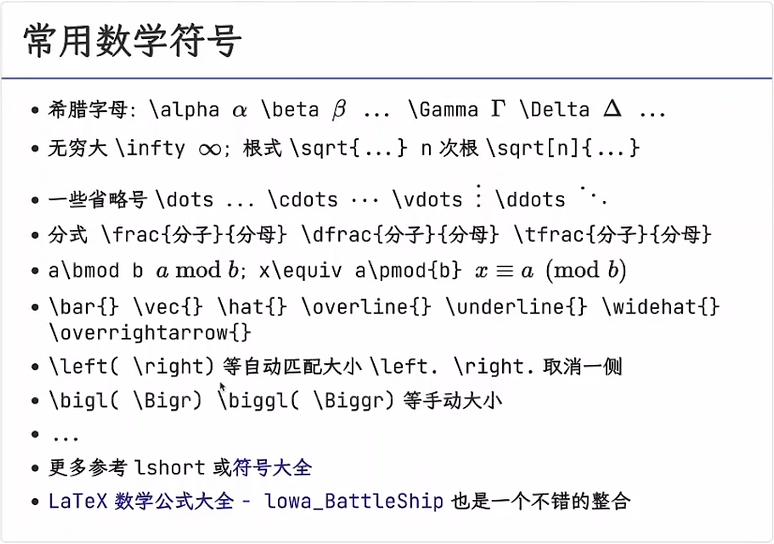
\includegraphics[scale=0.7]{pic/math-expression.png} \caption{frequently used math expression}\label{pic1}
\end{figure}
图中的\verb|\left(|和\verb|\right)|代表自动匹配括号大小。当然也可以用\verb|\left(|和\verb|\right.|这样的方式放弃一边的括号,但是绝对不能不匹配!(不能不写某一侧!)\\
\\
对齐模式:align/aligned对齐环境。可使用\verb|\notag|或者\verb|\align*|来取消编号。\\
aligned本身不自带数学环境!因此需要嵌套进入equation之类的环境才能使用!
\\
矩阵模式:参照另一份学习文档。
\subsection{standard of math expression}
\begin{enumerate}
    \item 特殊函数用特殊命令,或者是利用mathrm命令写为正体。能有专门的命令甚至都不能用mathrm!变量以外,全部正体!(尤其是各类算子)
    \item 正确使用displaystyle以及dfrac(性质一致)
    \item 注意区分\verb|\colon|以及手打冒号。前者被用于映射(一个标点),后者常被用于集合,例如$\{x:x=1\}$
    \item left和right的括号要经常用,只要内容不为一个字符高时,就必须要用自适配括号!
    \item 行间公式之间,如果有关联,不可直接加空行。
\end{enumerate}
\end{document}